\documentclass[border=10pt]{standalone} 
\usepackage{tikz}

\usetikzlibrary{calc}
\usetikzlibrary{arrows}
\usetikzlibrary{shadows}
\usetikzlibrary{patterns}
\usetikzlibrary{positioning}
\usetikzlibrary{shapes}
\usetikzlibrary{3d}
%\usetikzlibrary{automata}
\usetikzlibrary{fit}

\tikzset{block/.style={draw, text centered, fill=gray!10,drop shadow}}
\tikzset{connect/.style={draw, line width=1 pt}}

\begin{document}


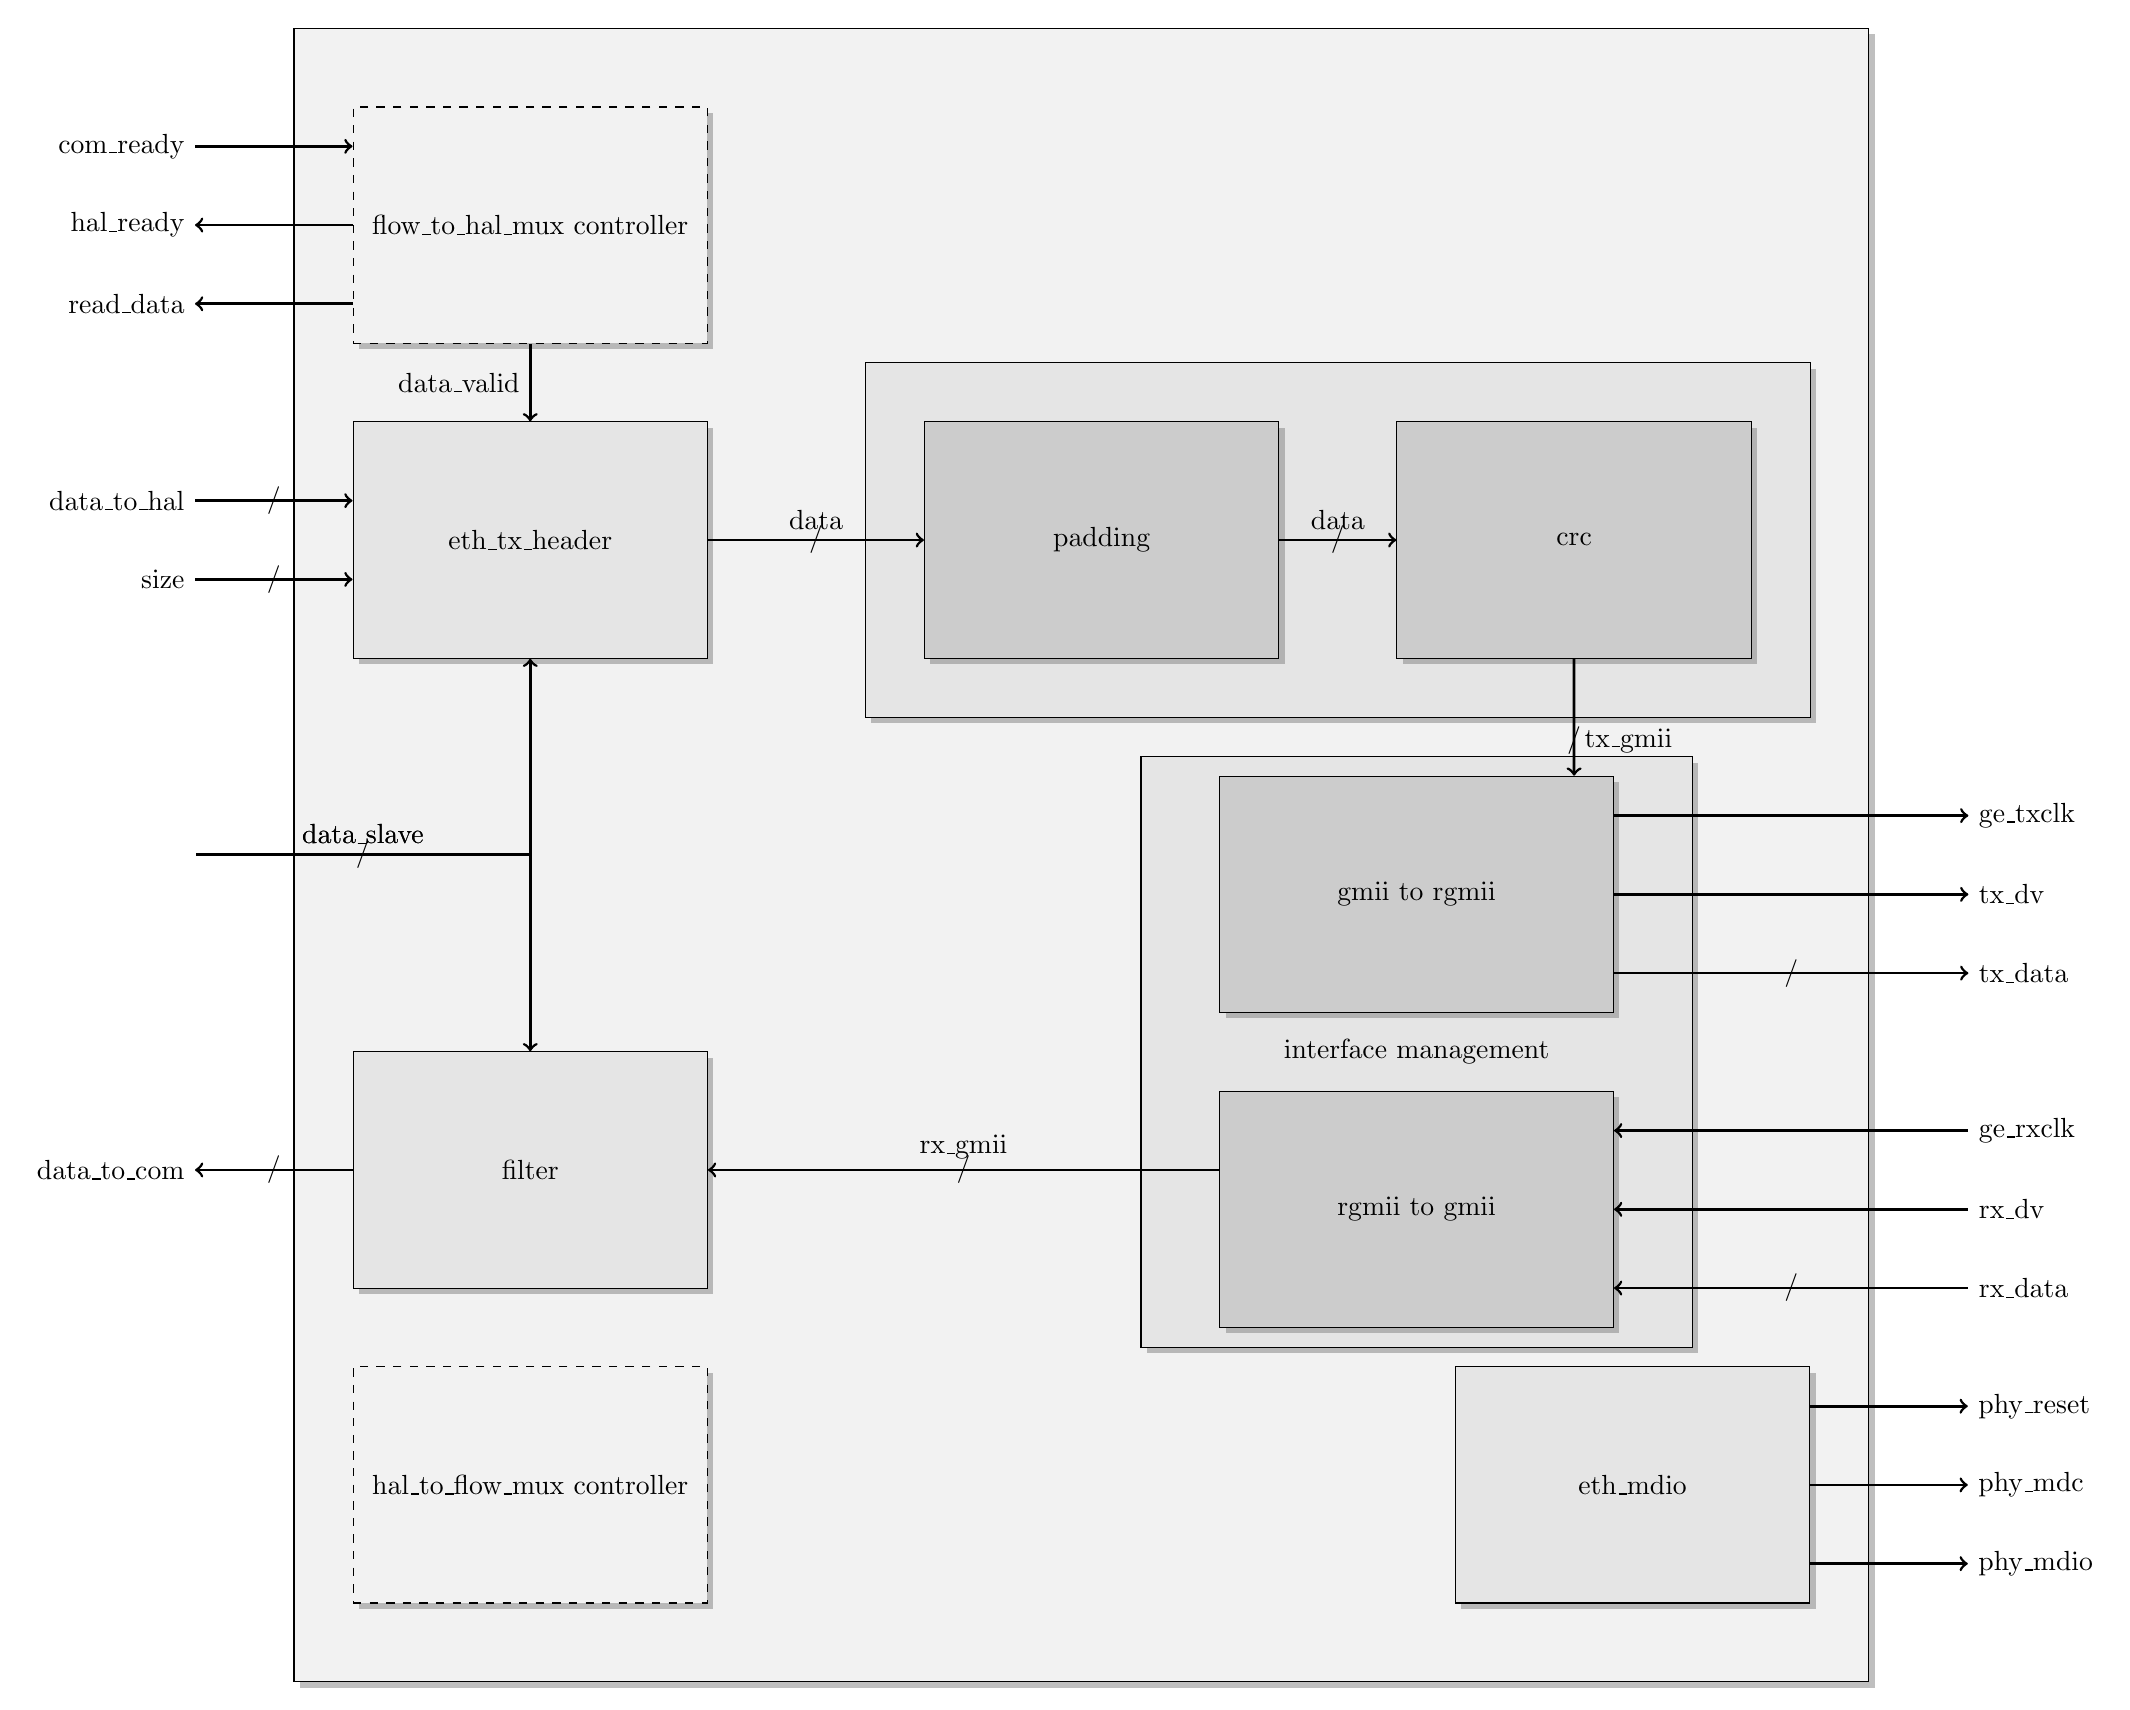
\begin{tikzpicture}




\node[block,minimum height=21cm,minimum width=20cm] (top) {};

%sub blocks
\node[block,minimum height=3cm,minimum width=4.5cm, fill=gray!20] (header) at([xshift=-7cm,yshift=4cm]top) {eth\_tx\_header};
\node[block,minimum height=3cm,minimum width=4.5cm, dashed] (controller) at([xshift=-7cm,yshift=8cm]top) {flow\_to\_hal\_mux controller};
\node[block,minimum height=3cm,minimum width=4.5cm, fill=gray!20] (filter) at([xshift=-7cm,yshift=-4cm]top) {filter};
\node[block,minimum height=3cm,minimum width=4.5cm, dashed] (controller2) at([xshift=-7cm,yshift=-8cm]top) {hal\_to\_flow\_mux controller};

\node[block,minimum height=3cm,minimum width=4.5cm, fill=gray!20] (mdio) at([xshift=7cm,yshift=-8cm]top) {eth\_mdio};

\node[block,minimum height=4.5cm,minimum width=12cm, fill=gray!20] (gemac) at([xshift=8cm]header.east) {};
\node[block,minimum height=3cm,minimum width=4.5cm, fill=gray!40] (crc) at([xshift=-3cm]gemac) {padding};
\node[block,minimum height=3cm,minimum width=4.5cm, fill=gray!40] (padding) at([xshift=3cm]gemac) {crc};

\node[block,minimum height=7.5cm,minimum width=7cm, fill=gray!20] (interface) at([xshift=1cm,yshift=-6.5cm]gemac) {interface management};
\node[block,minimum height=3cm,minimum width=5cm, fill=gray!40] (2rgmii) at([yshift=2cm]interface) {gmii to rgmii};
\node[block,minimum height=3cm,minimum width=5cm, fill=gray!40] (2gmii) at([yshift=-2cm]interface) {rgmii to gmii};

%mdio
\path[connect,->] ([yshift=1cm]mdio.east) -- ++(2cm,0) node[right]{phy\_reset};
\path[connect,->] ([yshift=0cm]mdio.east) -- ++(2cm,0) node[right]{phy\_mdc};
\path[connect,->] ([yshift=-1cm]mdio.east) -- ++(2cm,0) node[right]{phy\_mdio};

%flowtohal controller
\path[connect,<-] ([yshift=1cm]controller.west) -- ++(-2cm,0) node[left]{com\_ready};
\path[connect,->] ([yshift=0cm]controller.west) -- ++(-2cm,0) node[left]{hal\_ready};
\path[connect,->] ([yshift=-1cm]controller.west) -- ++(-2cm,0) node[left]{read\_data};
\path[connect,->] (controller.south) -- node[left]{data\_valid} (header.north);

%header / crc / padding
\path[connect,<-] ([yshift=0.5cm]header.west) -- node{/} ++(-2cm,0) node[left]{data\_to\_hal};
\path[connect,<-] ([yshift=-0.5cm]header.west) -- node{/} ++(-2cm,0) node[left]{size};
\path[connect,->] (header.east) -- node{/} node[above]{data} (crc.west);
\path[connect,->] (crc.east) -- node{/} node[above]{data} (padding.west);
\path[connect,->] (padding.south) -- node[pos=0.7]{/} node[right,pos=0.7]{tx\_gmii} ([xshift=2cm]2rgmii.north);

%interface
\path[connect,->] ([yshift=1cm]2rgmii.east) -- ++(4.5cm,0) node[right]{ge\_txclk};
\path[connect,->] ([yshift=0cm]2rgmii.east) --  ++(4.5cm,0) node[right]{tx\_dv};
\path[connect,->] ([yshift=-1cm]2rgmii.east) -- node{/} ++(4.5cm,0) node[right]{tx\_data};
\path[connect,<-] ([yshift=1cm]2gmii.east) -- ++(4.5cm,0) node[right]{ge\_rxclk};
\path[connect,<-] ([yshift=0cm]2gmii.east) --  ++(4.5cm,0) node[right]{rx\_dv};
\path[connect,<-] ([yshift=-1cm]2gmii.east) -- node{/} ++(4.5cm,0) node[right]{rx\_data};

%filter
\path[connect,->] ([yshift=0.5cm]2gmii.west) -- node{/} node[above]{rx\_gmii} (filter.east);
\path[connect,->] (filter.west) --node{/} ++(-2cm,0) node[left]{data\_to\_com};

%slave
\path[connect,<-] (filter.north) -- ([yshift=2.5cm]filter.north) --node[above]{data\_slave}node{/} ++(-4.25cm,0) ;
\path[connect,<-] (header.south) -- ([yshift=2.5cm]filter.north) --node[above]{data\_slave} ++(-4.25cm,0) ;

\end{tikzpicture}


\end{document}